    %%%%%%%%%%%%%%%%%%%%%%%%%%%%%%%%%%%%%%%%%
% Short Sectioned Assignment
% LaTeX Template
% Version 1.0 (5/5/12)
%
% This template has been downloaded from:
% http://www.LaTeXTemplates.com
%
% Original author:
% Frits Wenneker (http://www.howtotex.com)
%
% License:
% CC BY-NC-SA 3.0 (http://creativecommons.org/licenses/by-nc-sa/3.0/)
%
%%%%%%%%%%%%%%%%%%%%%%%%%%%%%%%%%%%%%%%%

%----------------------------------------------------------------------------------------
%	PACKAGES AND OTHER DOCUMENT CONFIGURATIONS
%----------------------------------------------------------------------------------------

\documentclass[paper=a4, fontsize=12pt, xcolor=dvipsnames]{scrartcl} % A4 paper and 11pt font size

% Biblatex

\usepackage[
style=nature,              % Zitierstil
isbn=false,                % ISBN nicht anzeigen, gleiches geht mit nahezu allen anderen Feldern
pagetracker=true,          % ebd. bei wiederholten Angaben (false=ausgeschaltet, page=Seite, spread=Doppelseite, true=automatisch)
maxbibnames=50,            % maximale Namen, die im Literaturverzeichnis angezeigt werden (ich wollte alle)
maxcitenames=3,            % maximale Namen, die im Text angezeigt werden, ab 4 wird u.a. nach den ersten Autor angezeigt
autocite=inline,           % regelt Aussehen für \autocite (inline=\parancite)
block=space,               % kleiner horizontaler Platz zwischen den Feldern
backref=false,              % Seiten anzeigen, auf denen die Referenz vorkommt
backrefstyle=three+,       % fasst Seiten zusammen, z.B. S. 2f, 6ff, 7-10
date=short,                % Datumsformat
hyperref=true,
backend = biber
]{biblatex}
\setlength{\bibitemsep}{1em}     % Abstand zwischen den Literaturangaben
\setlength{\bibhang}{2em}        % Einzug nach jeweils erster Zeile
\bibliography{report}  % Bibtex-Datei wird schon in der Preambel eingebunden
\usepackage{cmbright}
\usepackage[T1]{fontenc} % Use 8-bit encoding that has 256 glyphs
%\usepackage{fourier} % Use the Adobe Utopia font for the document - comment this line to return to the LaTeX default

\usepackage{amsmath,amsfonts,amsthm} % Math packages
\usepackage{pgfplots}
\usepackage{wrapfig}
\usepackage{color, colortbl}  

%\usepackage[pass,showframe]{geometry} % just to show the margins
%\usepackage{booktabs}
\usepackage{minted} % needs '-shell-escape' to compile

% Bibliographie auf deutsch
%\usepackage{harvard}
%\renewcommand{\harvardand}{und} 
%\usepackage{caption}
%\usepackage[usenames,dvipsnames]{xcolor}
\definecolor{gray1}{gray}{0.2}
\definecolor{gray2}{gray}{0.85}
\definecolor{LightCyan}{rgb}{0.88,0.8,1}
\usepackage[font={color=gray1},figurename=Fig.,labelfont={color=blue}]{caption}

\usepackage{titlesec}

\usepackage[utf8]{inputenc} 
%\usepackage[ngerman]{babel}

\usepackage{latexsym}
\usepackage{textcomp}
\usepackage{bm}% bold math
\usepackage{graphicx}
\usepackage{eso-pic}
\usepackage{caption}
\usepackage{subcaption}
\usepackage{verbatim}
\usepackage{epsfig}
\usepackage{framed,color}
\usepackage{placeins}   % FloatBarrier
\usepackage{float}
\usepackage{sidecap}
%\usepackage{float}      % adding boxes around figures
%\floatstyle{boxed}
%\restylefloat{figure}
\usepackage[usenames,dvipsnames]{pstricks}
\usepackage{epsfig}
\usepackage{tikz}
\usepackage{sectsty} % Allows customizing section commands
\usepackage{hyperref}

\hypersetup{
     colorlinks   = true,
     citecolor    = gray,
     linkcolor    = blue
}

\allsectionsfont{ \color{gray1} \normalfont\scshape} % Make all sections centered, the default font and small caps

\usepackage{fancyhdr} % Custom headers and footers
\pagestyle{fancy} % Makes all pages in the document conform to the custom headers and footers

\renewcommand{\headrulewidth}{0.0pt} % Remove header underlines
\renewcommand{\footrulewidth}{0pt} % Remove footer underlines



\numberwithin{equation}{section} % Number equations within sections (i.e. 1.1, 1.2, 2.1, 2.2 instead of 1, 2, 3, 4)
\numberwithin{figure}{section} % Number figures within sections (i.e. 1.1, 1.2, 2.1, 2.2 instead of 1, 2, 3, 4)
\numberwithin{table}{section} % Number tables within sections (i.e. 1.1, 1.2, 2.1, 2.2 instead of 1, 2, 3, 4)

\setlength\parindent{0pt} % Removes all indentation from paragraphs - comment this line for an assignment with lots of text
\setcapindent{1cm} 

%----------------------------------------------------------------------------------------
%	TITLE SECTION
%----------------------------------------------------------------------------------------
\title{
\normalfont \normalsize 
\textsc{Albert-Ludwigs-University Freiburg} \\ [25pt] % Your university, school and/or department name(s)
\horrule{0.5pt} \\[0.4cm] % Thin top horizontal rule
\huge \textsc{Analysis of $Z^0$ decays} \\ % The assignment title
\horrule{2pt} \\[0.5cm] % Thick bottom horizontal rule
}

\author{Friedrich Schüßler and Volker Karle} % Your name

\date{\normalsize\today} % Today's date or a custom date
\DeclareGraphicsExtensions{.pdf,.png,.jpg}

%--------------------------------------------------------------------------------------------
% New Commands
%--------------------------------------------------------------------------------------------
\newcommand{\horrule}[1]{\color{gray1}\rule{\linewidth}{#1}} % Create horizontal rule command with 1 argument of height


\begin{document}

\color{gray1}
\maketitle
\begin{center}
 
\includegraphics[width=0.6\linewidth]{figures/unifreiburg}
\end{center}
\thispagestyle{empty}
\newpage
    {\pagestyle{plain}
    \thispagestyle{empty}
    \tableofcontents
    \thispagestyle{empty}
    \cleardoublepage}
\newpage


%----------------------------------------------------------------------------------------
%	CONTENT
%----------------------------------------------------------------------------------------
\setcounter{page}{1}


% This file contains all the new commands defined 
% in order to facilitate the writing of the latex code. 
% It has to be loaded into the main .tex file at the beginning!

\newcommand{\nn}{\nonumber \\}
\newcommand{\beq}{\begin{equation}}
\newcommand{\eeq}{\end{equation}}
\newcommand{\beqn}{\begin{equation*}}   % equation without numbering
\newcommand{\eeqn}{\end{equation*}}
\newcommand{\bea}{\begin{eqnarray}}
\newcommand{\eea}{\end{eqnarray}}
\newcommand{\bean}{\begin{eqnarray*}}
\newcommand{\eean}{\end{eqnarray*}}
\newcommand{\bit}{\begin{itemize}}
\newcommand{\eit}{\end{itemize}}

\newcommand{\E}{\mathbf{E}}
\newcommand{\D}{\mathbf{D}}
\newcommand{\B}{\mathbf{B}}



\section{Analysis of technical devices}
\subsection{Scintillators without amplification}
test
\newpage


\setcounter{page}{1}
Nothing to see here. Pass on.
\section{Analysis and results}
\label{sec:analysis}

\subsection{Calibration of PVC scintillator}
\label{sub:calibration}
The purpose of this section is to calibrate the channels to known energies, in our case
\begin{itemize}
\item $^{22}$Na Compton edge 1: 341 keV
\item $^{22}$Na Compton edge 2: 1064 keV
\item $^{137}$Cs Compton edge: 477 keV
\end{itemize}
First we fit the two Compton edges of the $^{22}$Na sample. The result is
channel $108 \pm 2$ and $414 \pm 4$ with a correlation of about 50\%, see
figure~\ref{fig:calib_ps_na}.

\begin{figure}[htpb]
    \centering
    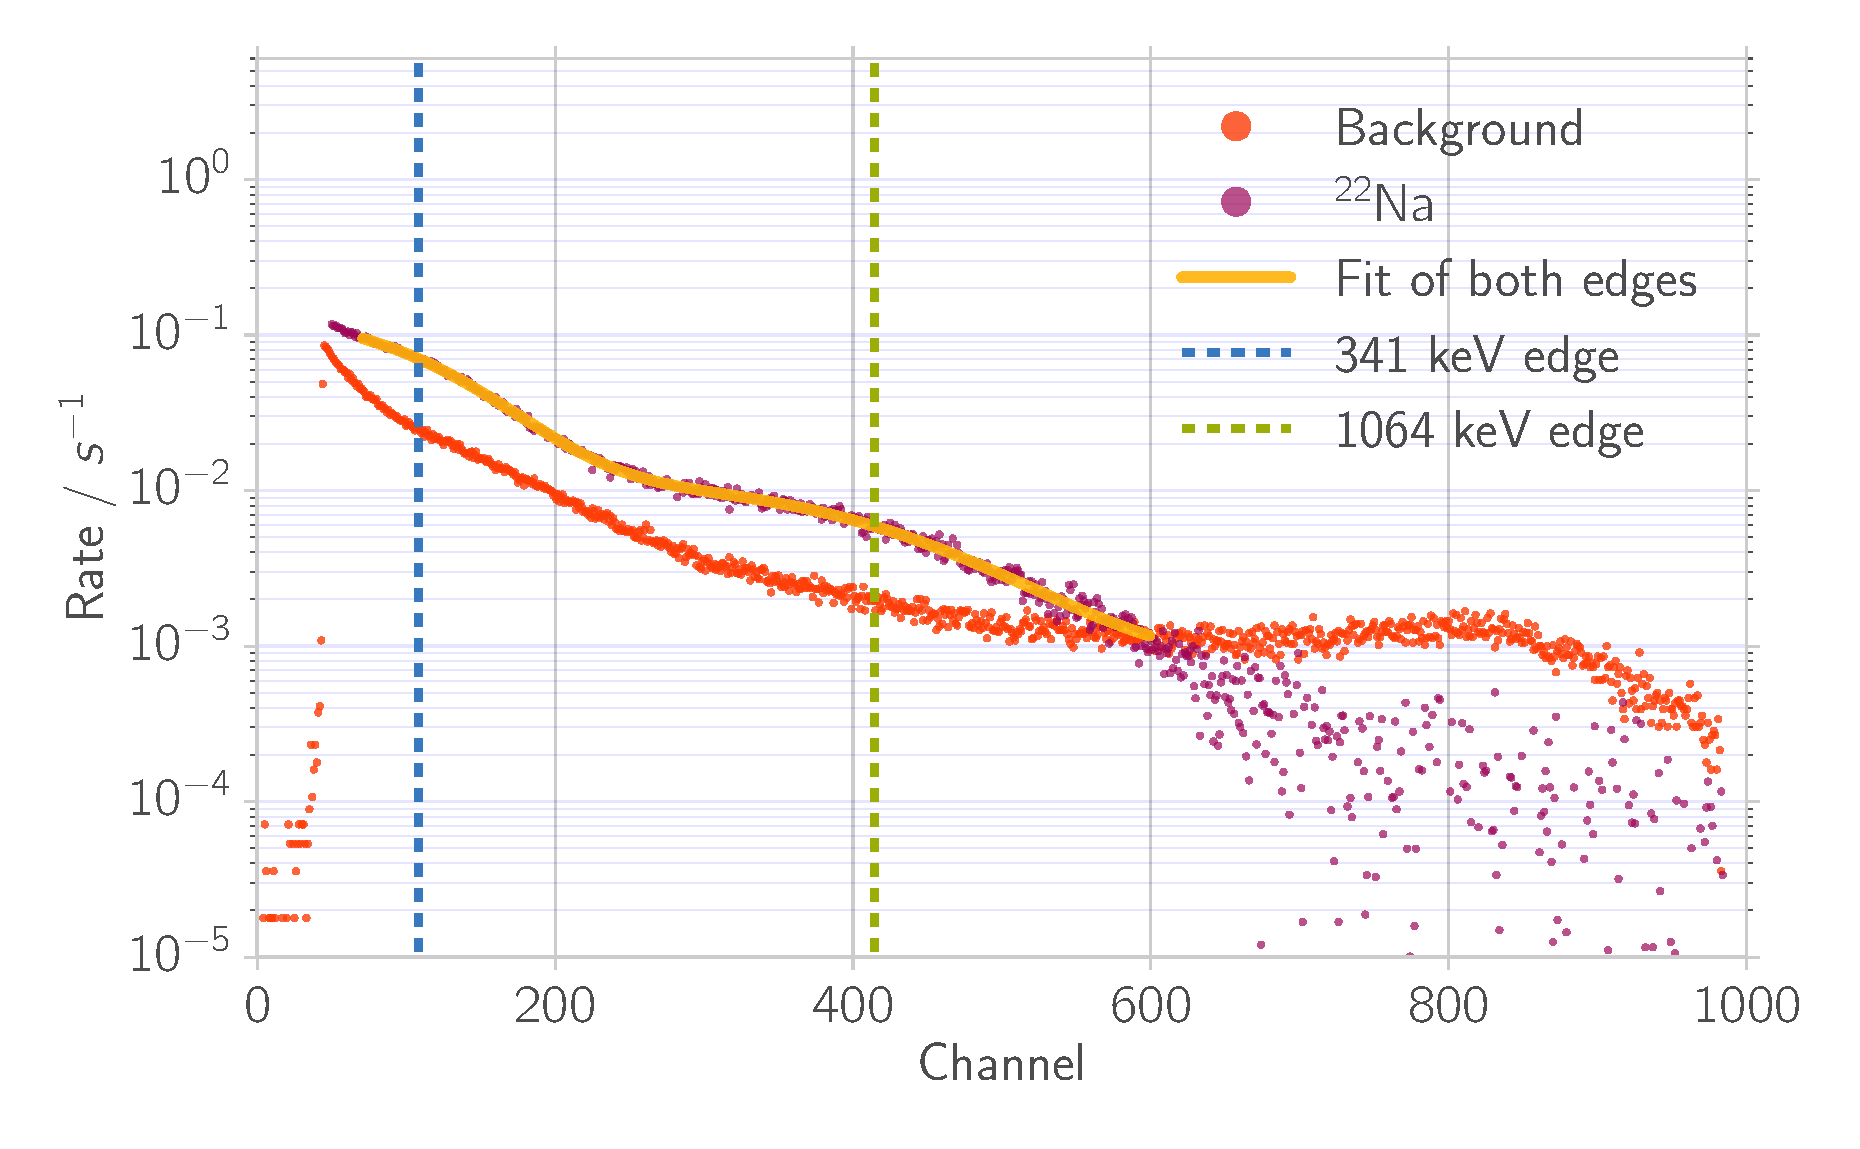
\includegraphics[width=0.9\linewidth]{./analysis/figures/calib_ps_na}
    \caption{Calibration of the PVC scintillator with $^{22}$Na sample (measurement time
    16.5 h) with refined background (measurement time 15.6h). Notice that the rate is 
    only fitted for the section in which the background is smaller than the sample. We
    subtracted the background rate at each channel for the sample in order not to fit the 
    behavior of the noise. The error of the two Compton edges is large (see text) coming
    from the fit and their high correlation coefficient.}
\label{fig:calib_ps_na}
\end{figure}
For the $^{137}$Cs sample we found the Compton edge at channel $178.9 \pm 0.3$ 
(notice the much smaller error compared to the $^{22}$Na sample), 
see figure~\ref{fig:calib_ps_cs} for the data and the fit.
\begin{figure}[htpb]
    \centering
    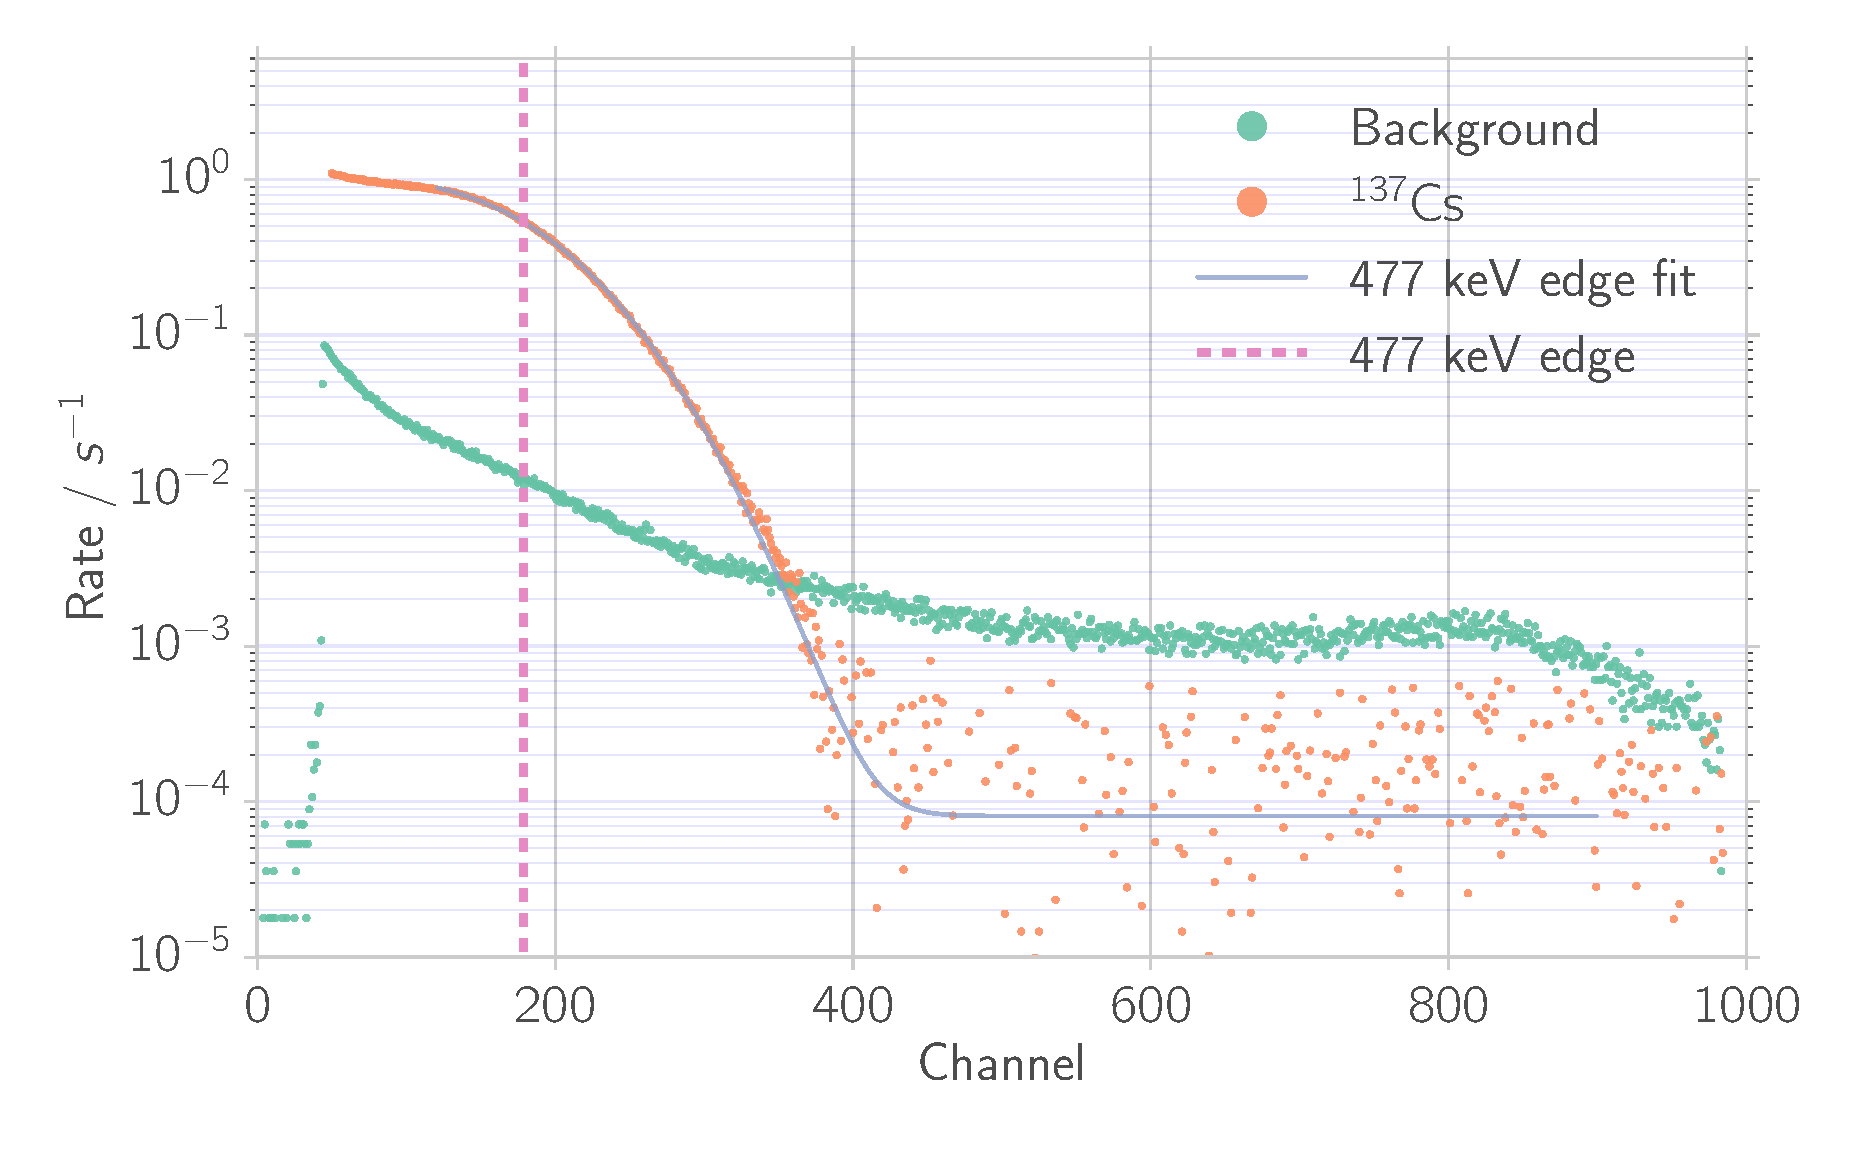
\includegraphics[width=0.9\linewidth]{./analysis/figures/calib_ps_cs}
    \caption{Calibration of the PVC scintillator with $^{137}$Cs sample. Measurement time
    6 h. We subtracted the background rate at each channel. }
\label{fig:calib_ps_cs}
\end{figure}

\begin{figure}[htpb]
    \centering
    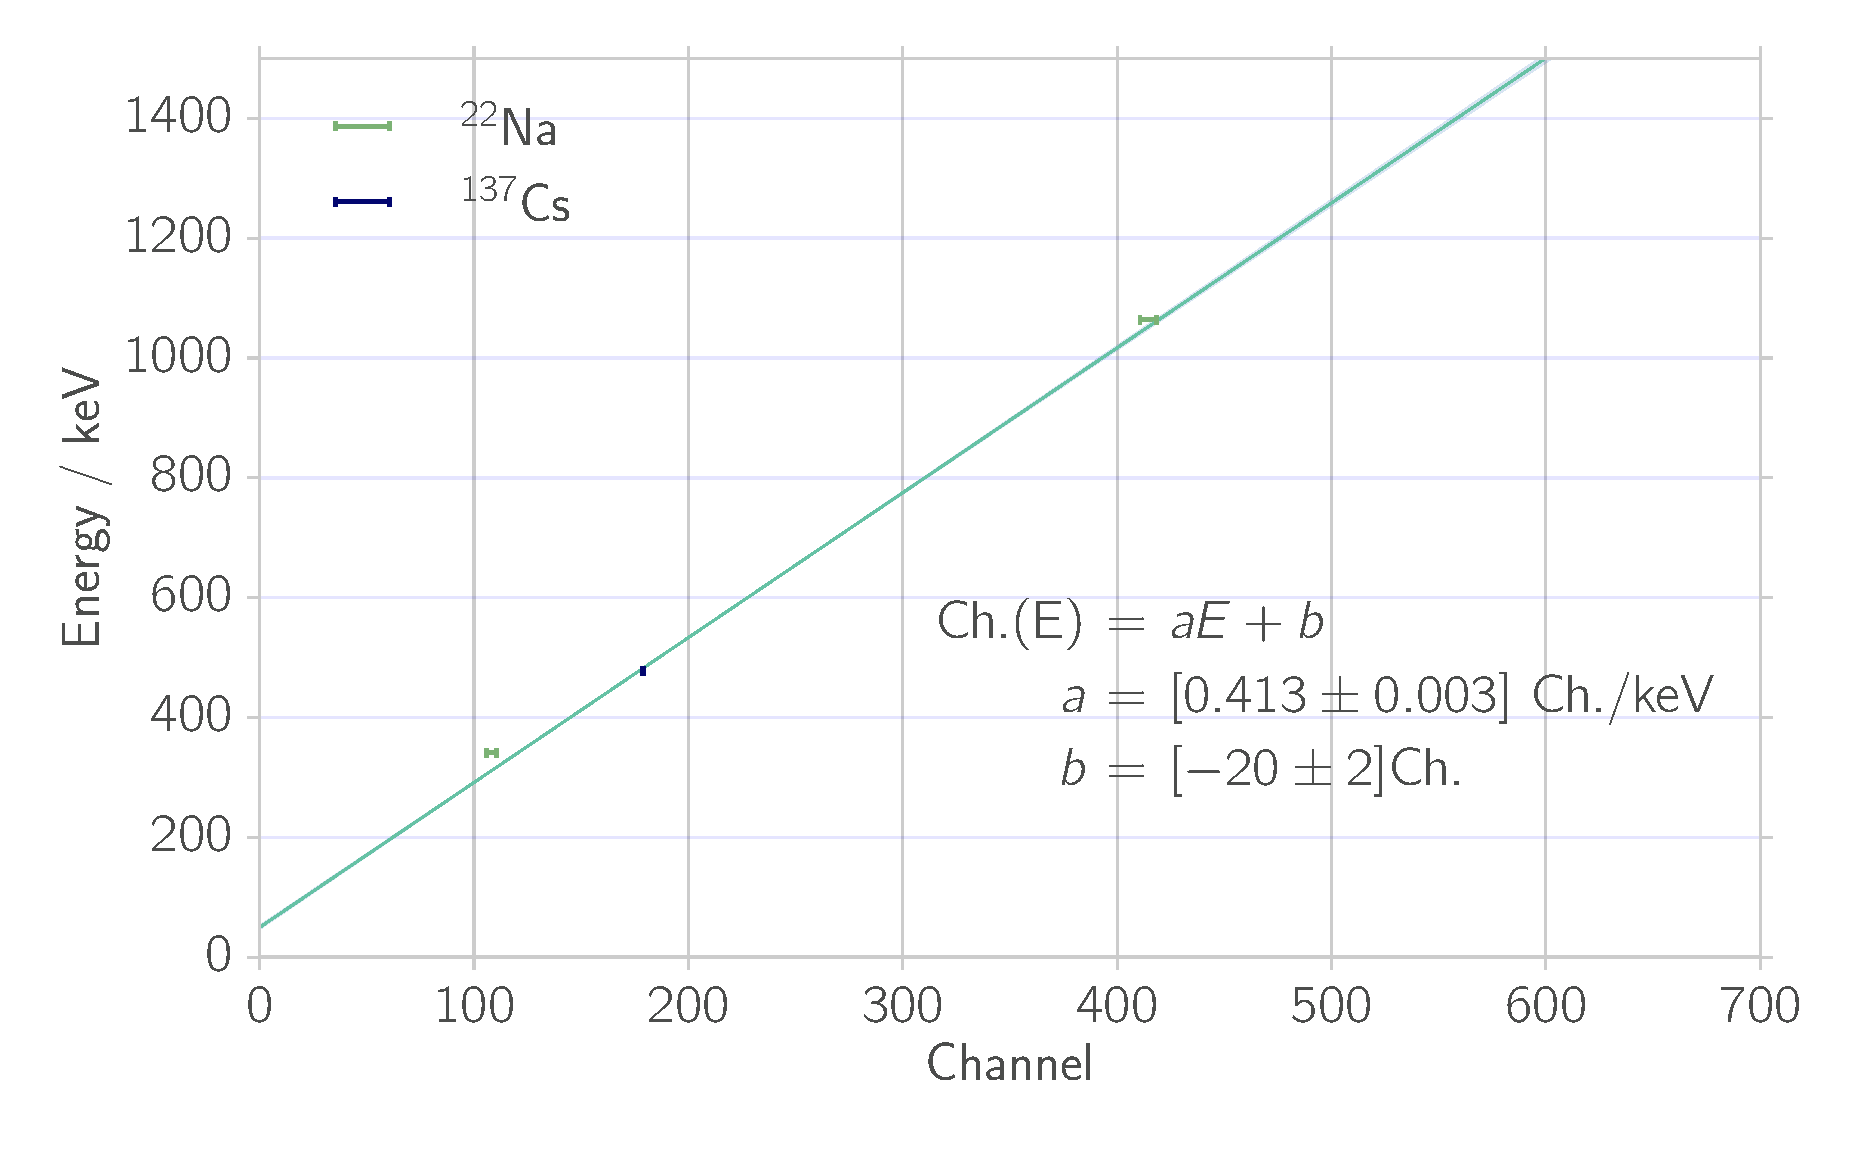
\includegraphics[width=0.9\linewidth]{./analysis/figures/calibration_ps_linear_fit}
    \caption{This is the result of the three Compton edges. We will use this calibration
    for all the following calculations. Note that statements about the error and linearity of the MCA 
    are not possible due to the low number of data points}
\label{fig:calibration_ps_linear_fit}
\end{figure}
The final result of the linear calibration can be seen in
figure~\ref{fig:calibration_ps_linear_fit}.

\subsection{Calibration of NaI scintillator}

\label{sub:calibration_of_na_scintillator}
As in the last section we calculate a calibration, this time for the NaI scintillator. The
first figure~\ref{fig:histo_na_137cs} shows the spectrum of the $^{136}$Cs sample 
whereas the data for
$^{22}Na$ can be seen in figure~\ref{fig:histo_na_22na} and figure~\ref{fig:histo_na_22na2}.
The results of the peak fits as well as literature values are displayed in the tables~\ref{tab:peaks_cs_ps}
and \ref{tab:peaks_na_ps} for each of the two samples. The literature values are fitted over peak positions, see 
figure~\ref{fig:calibration_na_linear_fit}, in order to yield a calibration. 
\begin{table}[htpb]
    \centering
    \caption{Peaks and fitting results of $^{136}$Cs.}
\label{tab:peaks_cs_ps}
    \begin{tabular}{lll}
        \rowcolor{LightCyan} Name &Energy & Channel \\ 
        Photo peak & 662 keV & $8040.59 \pm 0.03$\\ 
        Compton edge & 477 keV & $5720 \pm 4$\\  
        Escape peak & 183 keV & $2510 \pm 12$
    \end{tabular}
\end{table}

\begin{figure}[htpb]
    \centering
    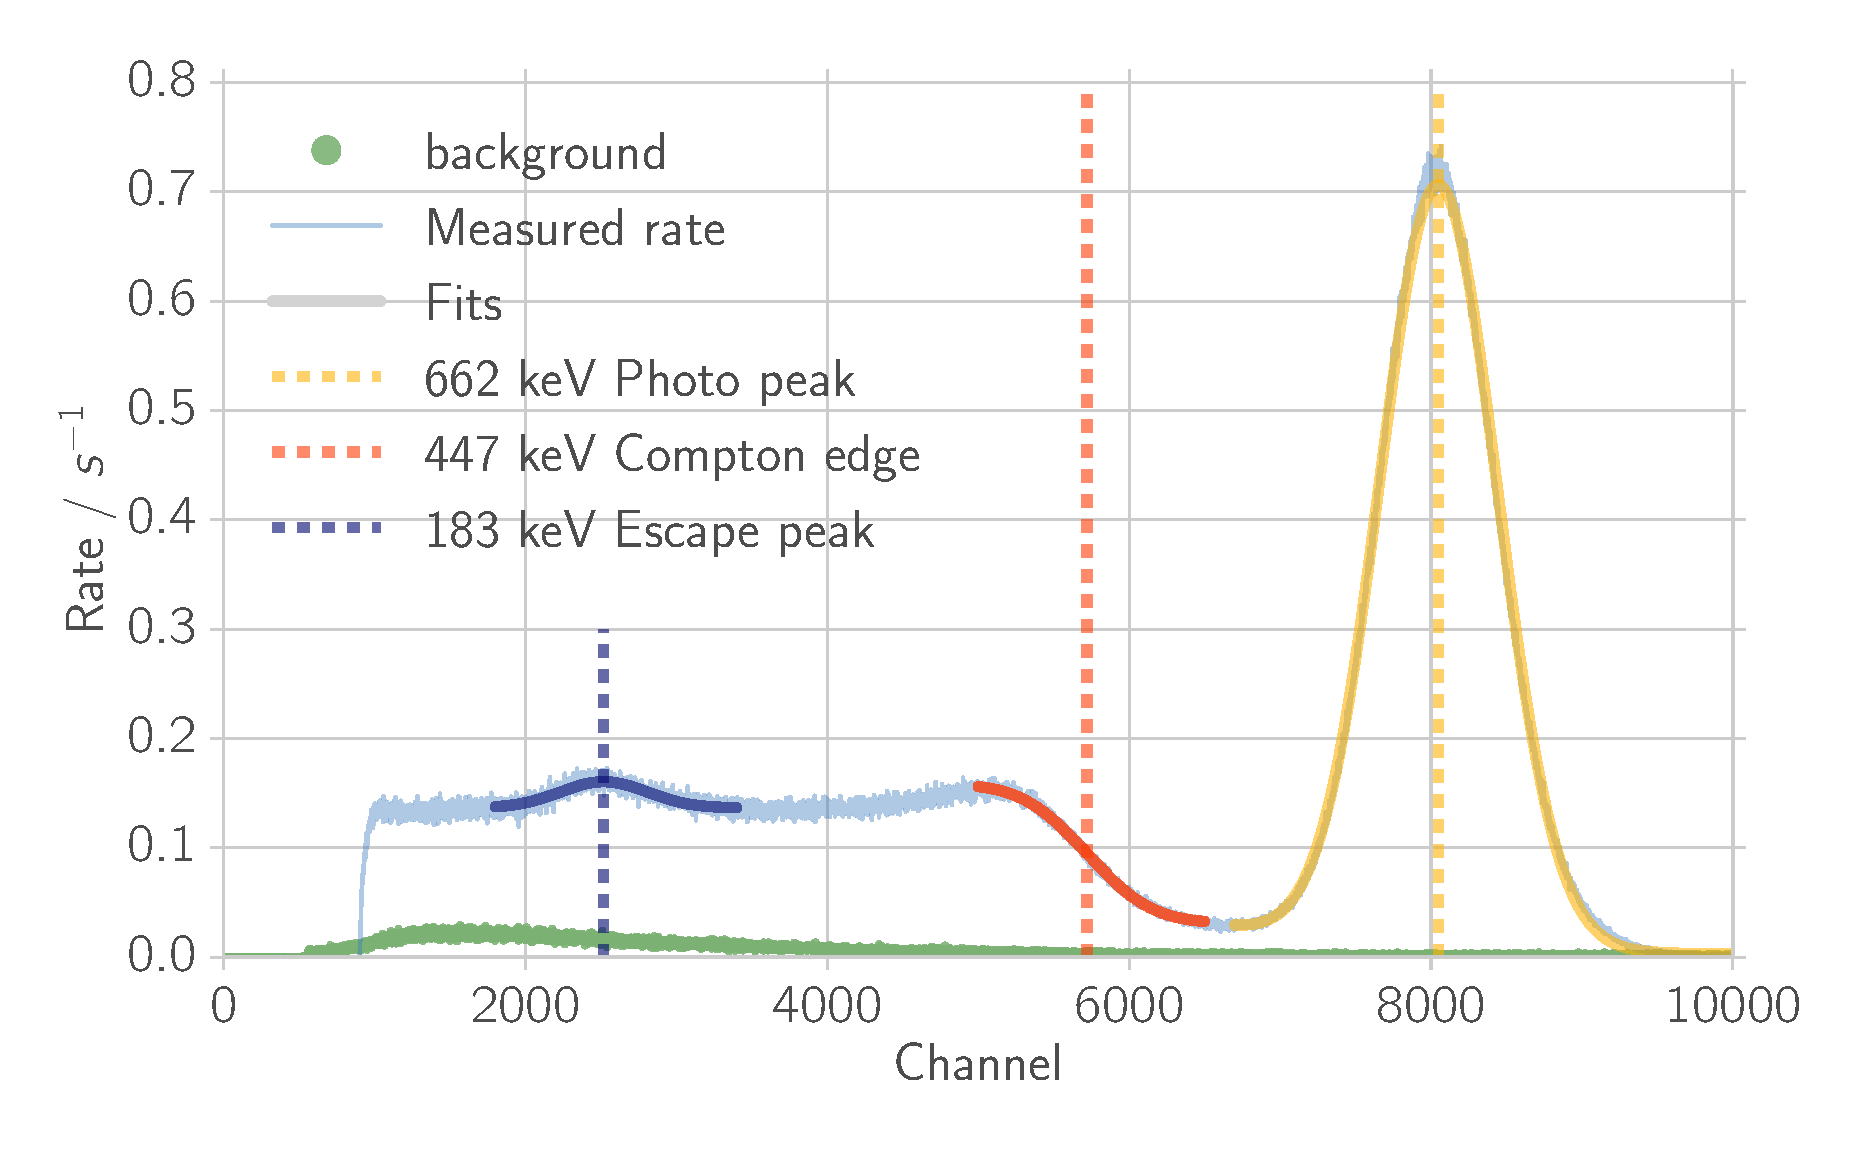
\includegraphics[width=0.9\linewidth]{./analysis/figures/histo_na_137cs}
    \caption{Calibration of the NaI scintillator using $^{137}$Cs sample (measurement
    time 2.7h) with refined background (measurement time 1h). }
\label{fig:histo_na_137cs}
\end{figure}

\begin{figure}[htpb]
    \centering
    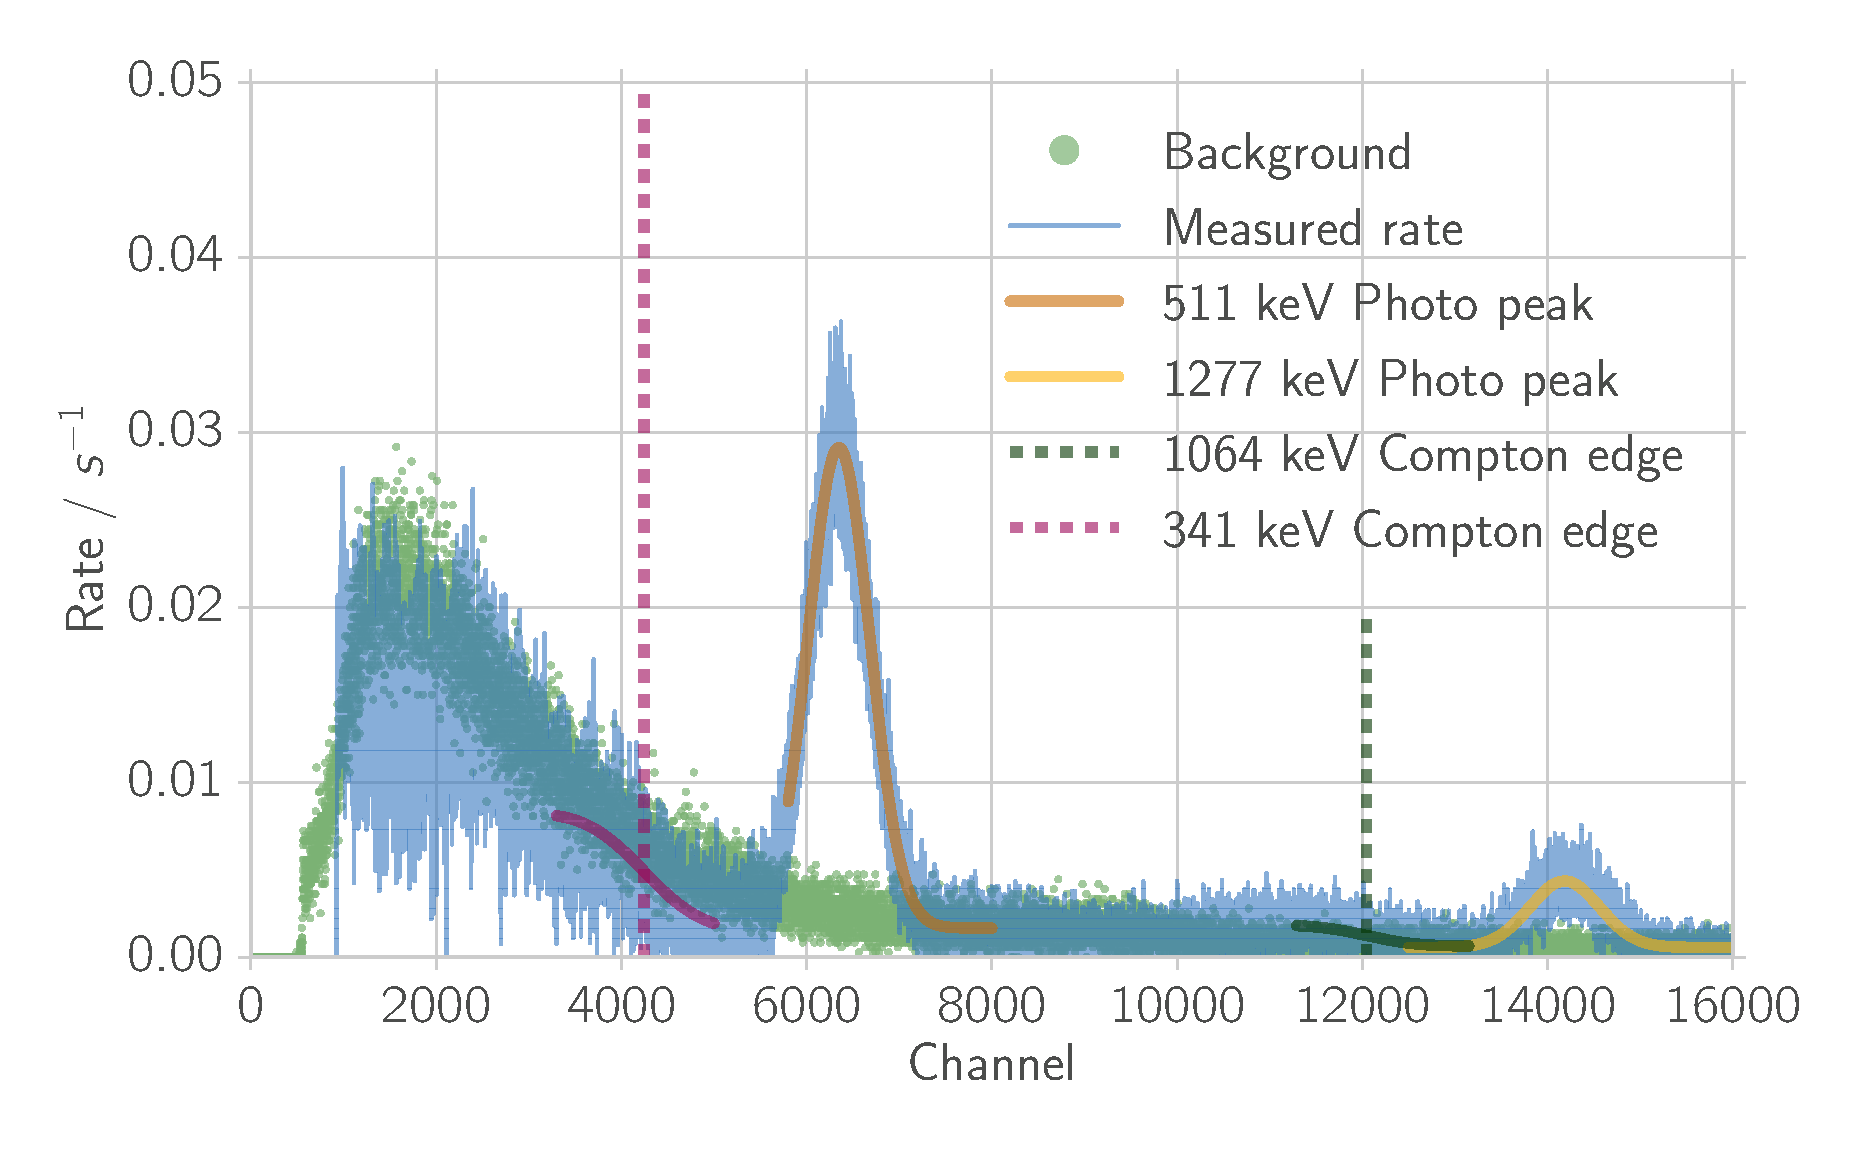
\includegraphics[width=0.9\linewidth]{./analysis/figures/histo_na_22na}
    \caption{Calibration of the NaI scintillator using $^{22}$Na sample (measurement
        time about 1h) with refined background (same as in figure~\ref{fig:histo_na_137cs},
        measurement time 1h). }
\label{fig:histo_na_22na}
\end{figure}

\begin{figure}[htpb]
    \centering
    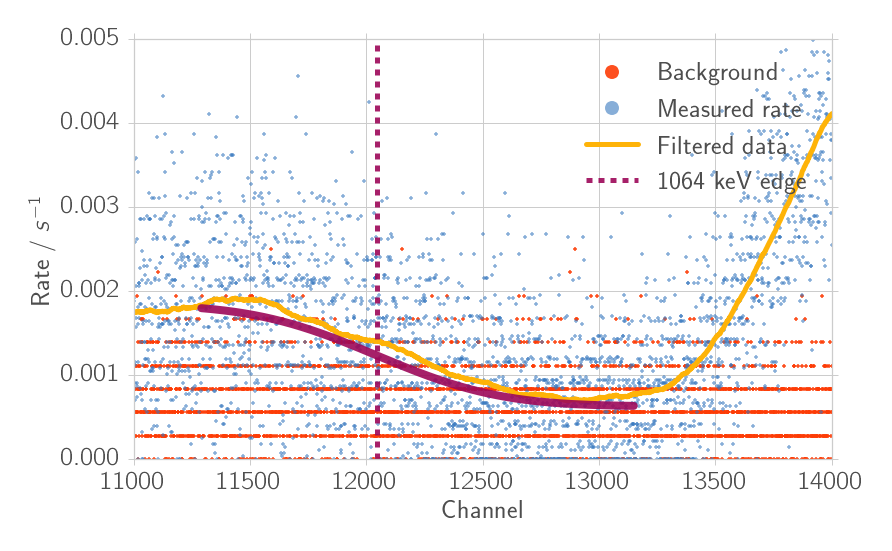
\includegraphics[width=0.9\linewidth]{./analysis/figures/histo_na_22na2}
    \caption{Enlargement of the critical area of the Compton edge of
    figure~\ref{fig:histo_na_22na}.     
    The red line is a Savitzky-Golay filter 
    with a width of 1001 points and a fourth
    degree polynomial applied to the data (see~\cite{scipy} for reference) in order
    to see the slope of the curve. The least-squares fit uses the real data, though.
}
\label{fig:histo_na_22na2}
\end{figure}

\begin{table}[htpb]
    \centering
    \caption{Peaks and fitting results of $^{22}$Na. As it is also visible in the figure
    of the leasts-squares fit~\ref{fig:calibration_na_linear_fit} the errors on the
    Compton edges are much higher than those of the Photo peaks. This is due to the high
    degree of uncertainty of the particular edge resulting from the fit. However, the 
    uncertainty of the linear fit is much less in the end.}
\label{tab:peaks_na_ps}
\begin{tabular}{lll}
    \rowcolor{LightCyan} Name &Energy & Channel \\ 
       1. Photo peak& 511 keV & $6347 \pm 3$ \\ 
       2. Photo peak& 1277 keV & $14180 \pm 20 $\\
       1. Compton edge& 341 keV& $4000 \pm 2000$\\
       2. Compton edge& 1064 keV & $12000 \pm 4000$
    \end{tabular}
\end{table}

\begin{figure}[htpb]
    \centering
    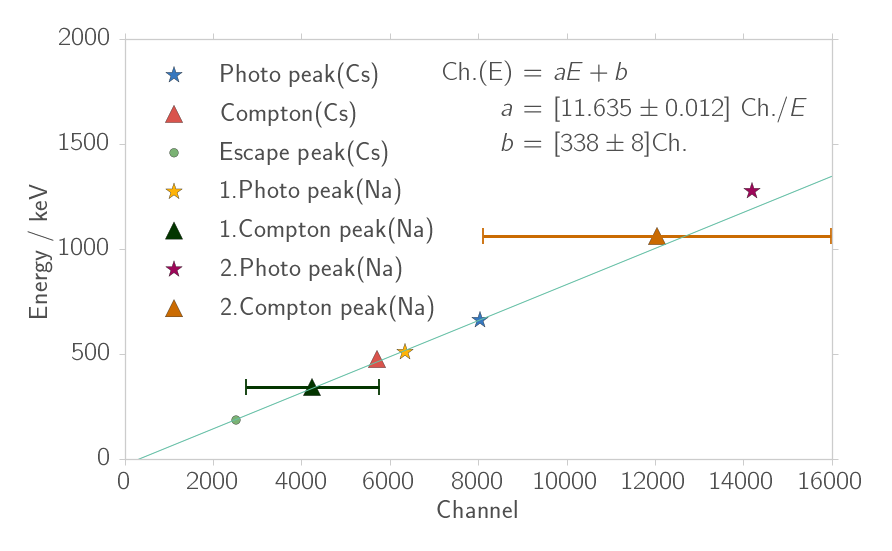
\includegraphics[width=0.9\linewidth]{./analysis/figures/calibration_na_linear_fit}
    \caption{All peaks measured by the NaI scintillator with the respective linear fit. The errors on 
        most of the peaks are too small to be shown, only the Compton peaks of $^{22}$Na show
        an exorbitant error. The second photo peak ($^{22}$Na sample) seems to be quite apart from
    the result of the other values; this might be due to a general systematic error.}
\label{fig:calibration_na_linear_fit}
\end{figure}
\clearpage
\subsection{Energy conservation}
\label{sub:energy_conservation}
In this section we work out the dependence of the energy with respect to the scattered
angle. Figure~\ref{fig:coin_ps_background} shows the background (with
coincident setup but without sample) and random coincidences.
We subtract the background from our data before pursuing the analysis.
This will include evaluating a number of different measurements; we will
only show two example figures for each detector 
(figures~\ref{fig:coin_ps_90} and~\ref{fig:coin_ps_15} for the PVC scintillator and 
~\ref{fig:coin_na_90} and~\ref{fig:coin_na_30} for the NaI scintillator). The main
result is summarized in figure~\ref{fig:coin_na_90}. It shows the expectation values of
the energy, dependent on different scattering angles $\theta$.


\begin{figure}[htpb]
    \centering
    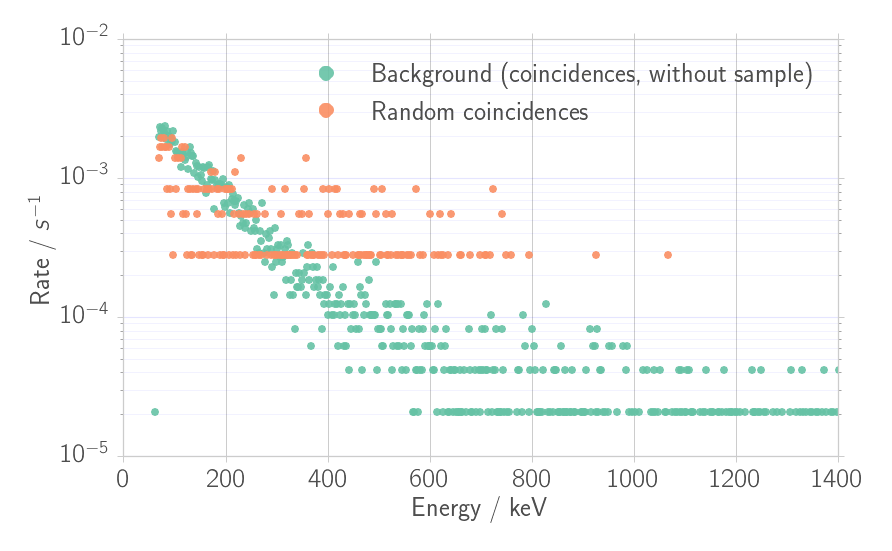
\includegraphics[width=0.9\linewidth]{./analysis/figures/coin_background_random}
    \caption{Background and random coincidences of the PVC scintillator. 
        The background is measured in coincident setup for 13.4h, the random coincidences are 
    measured with the $^{137}$Cs sample inserted (measurement time 1h).}
\label{fig:coin_ps_background}
\end{figure}

\begin{figure}[htpb]
    \centering
    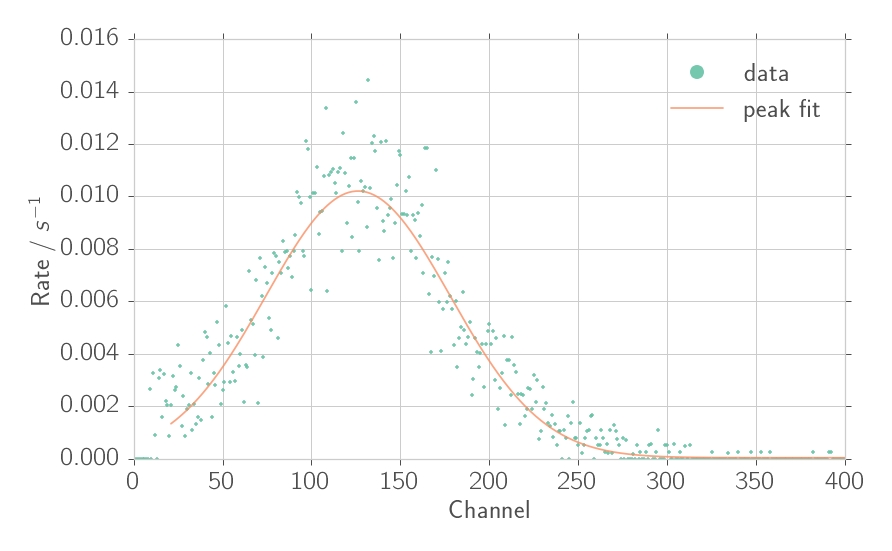
\includegraphics[width=0.9\linewidth]{./analysis/figures/coin_ps_90}
    \caption{\textbf{Energy of electrons:}
    Rate of coincident events of PVC scintillator at angle of $\theta = 90^\circ$ 
        (measurement time 1h). The distribution 
    was approximated with a Gaussian distribution. }
\label{fig:coin_ps_90}
\end{figure}

\begin{figure}[htpb]
    \centering
    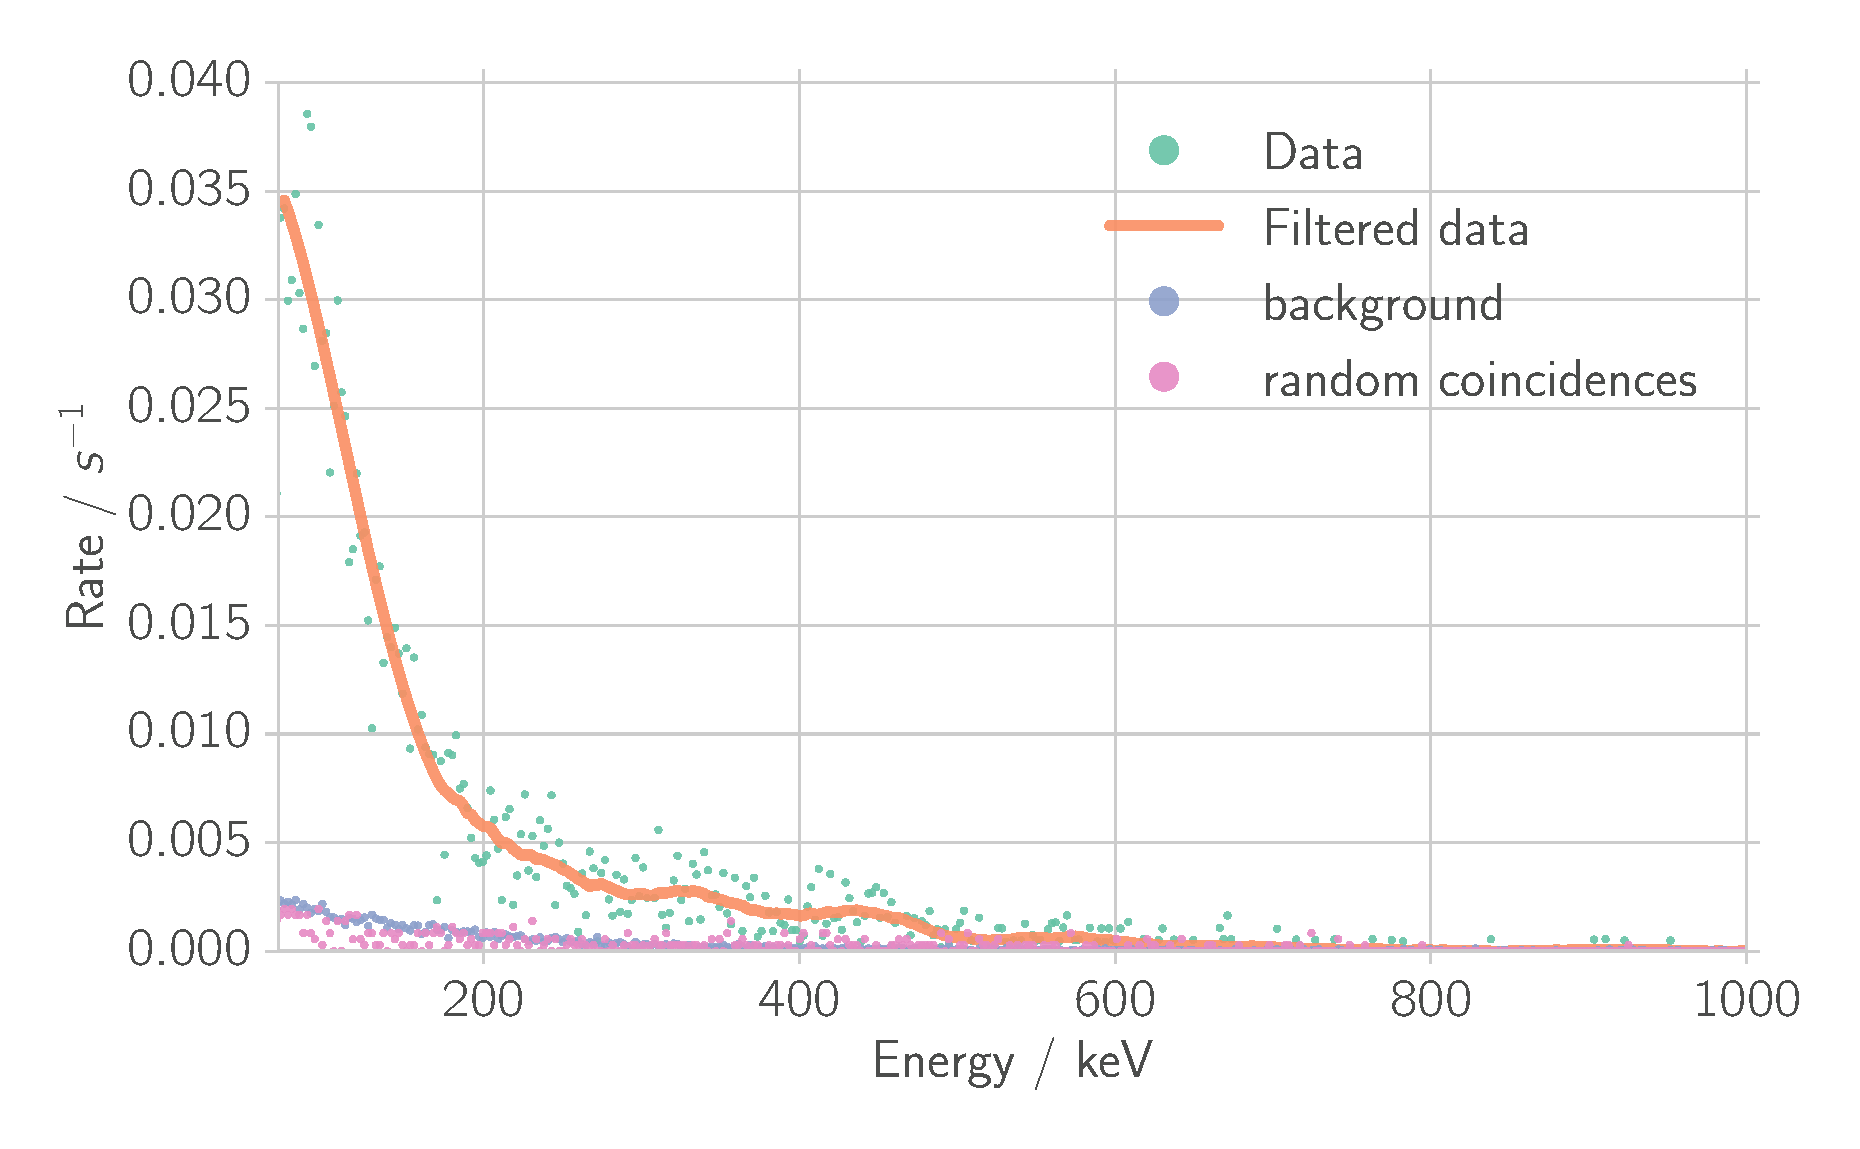
\includegraphics[width=0.9\linewidth]{./analysis/figures/coin_ps_15_filter_}
    \caption{\textbf{Energy of electrons:}
        Rate of coincident events of 
        PVC scintillator at angle of $\theta = 15^\circ$.
        In this figure we used, unlike at higher angles, applying the Savitzky-Golay filter
        with a width of 81 points and a fourth
        degree polynomial (see~\cite{scipy} for reference). This was done for 
        angles $\theta = 15^\circ$ up to $\theta = 60^\circ$.}
\label{fig:coin_ps_15}
\end{figure}

\begin{figure}[htpb]
    \centering
    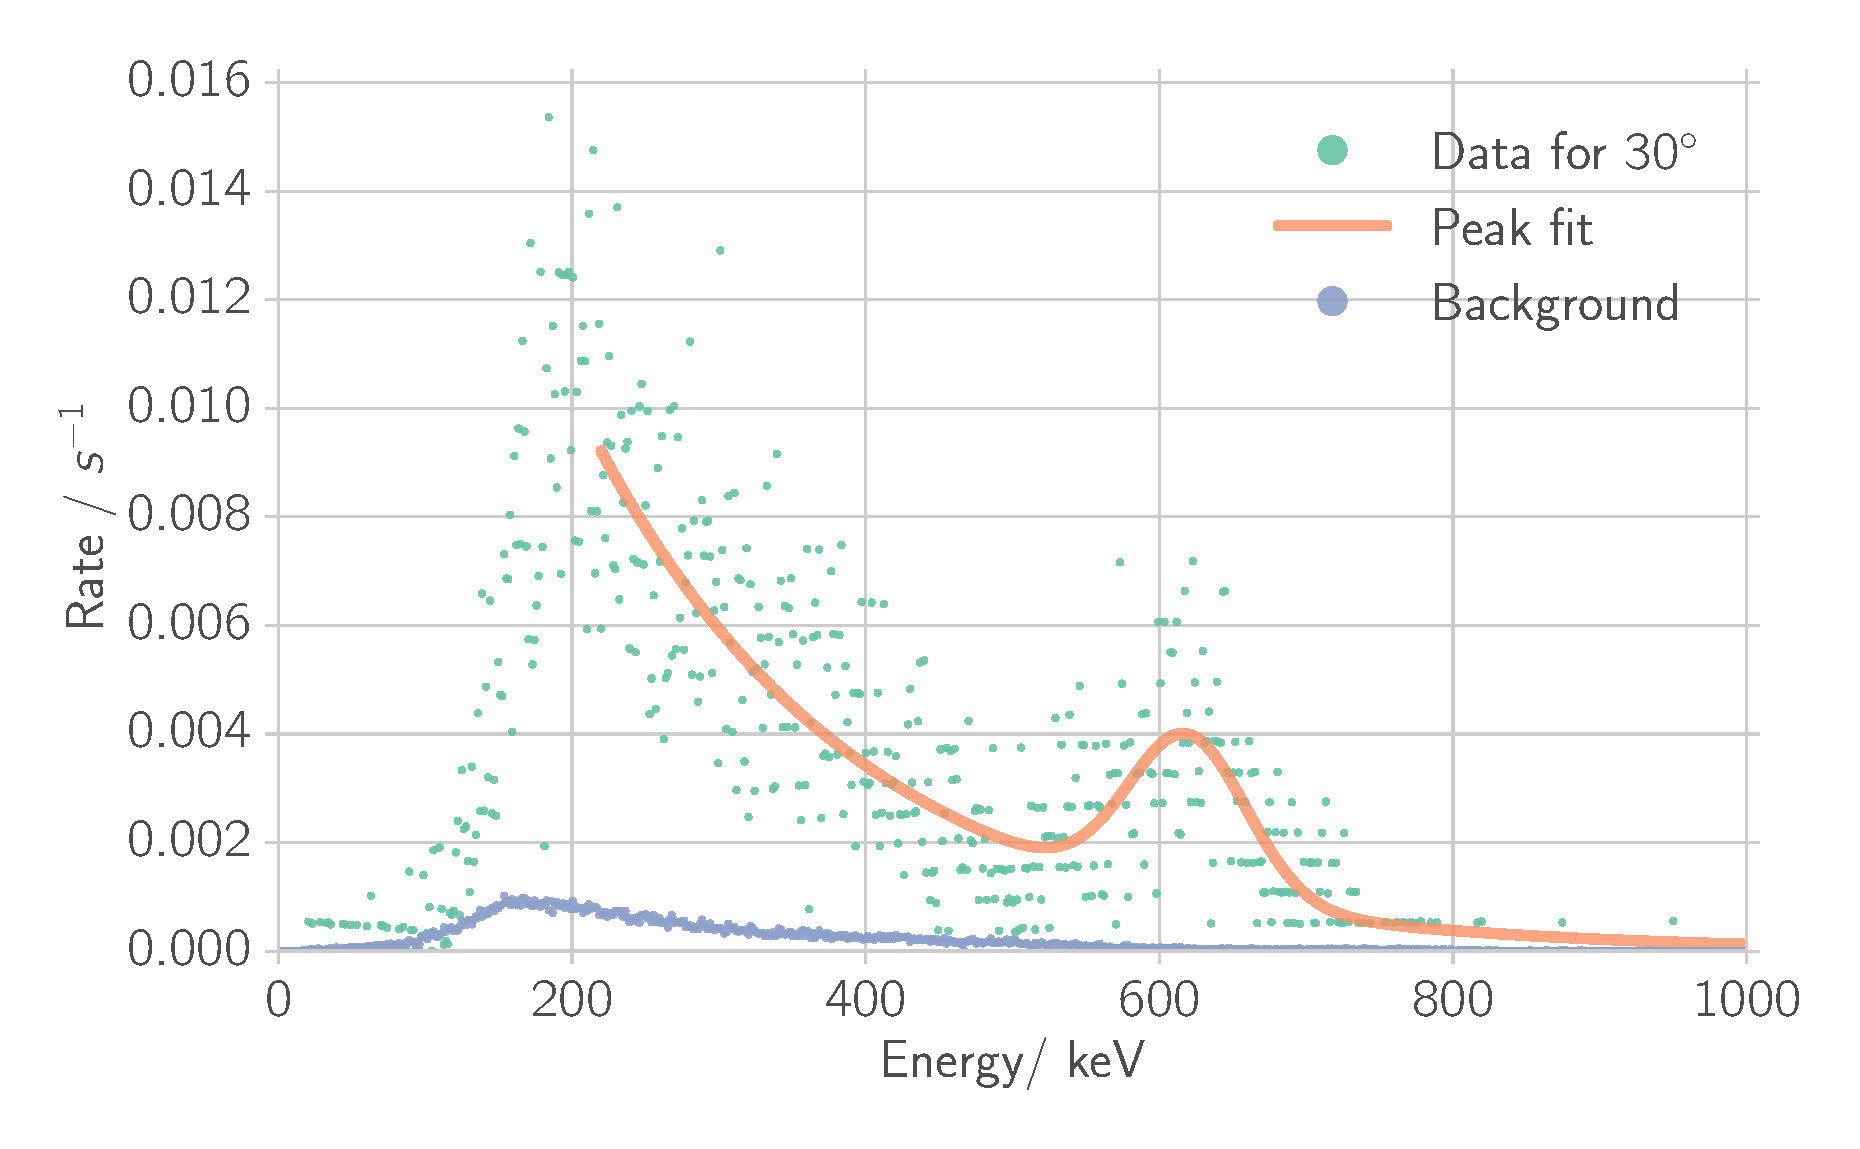
\includegraphics[width=0.9\linewidth]{./analysis/figures/coin_na_30}
    \caption{\textbf{Energy of photons:} Rate of coincident events of 
        NaI scintillator at angle of $\theta = 15^\circ$. The photo peak was approximated
        with a Gaussian distribution.}
\label{fig:coin_na_30}
\end{figure}




\begin{figure}[htpb]
    \centering
    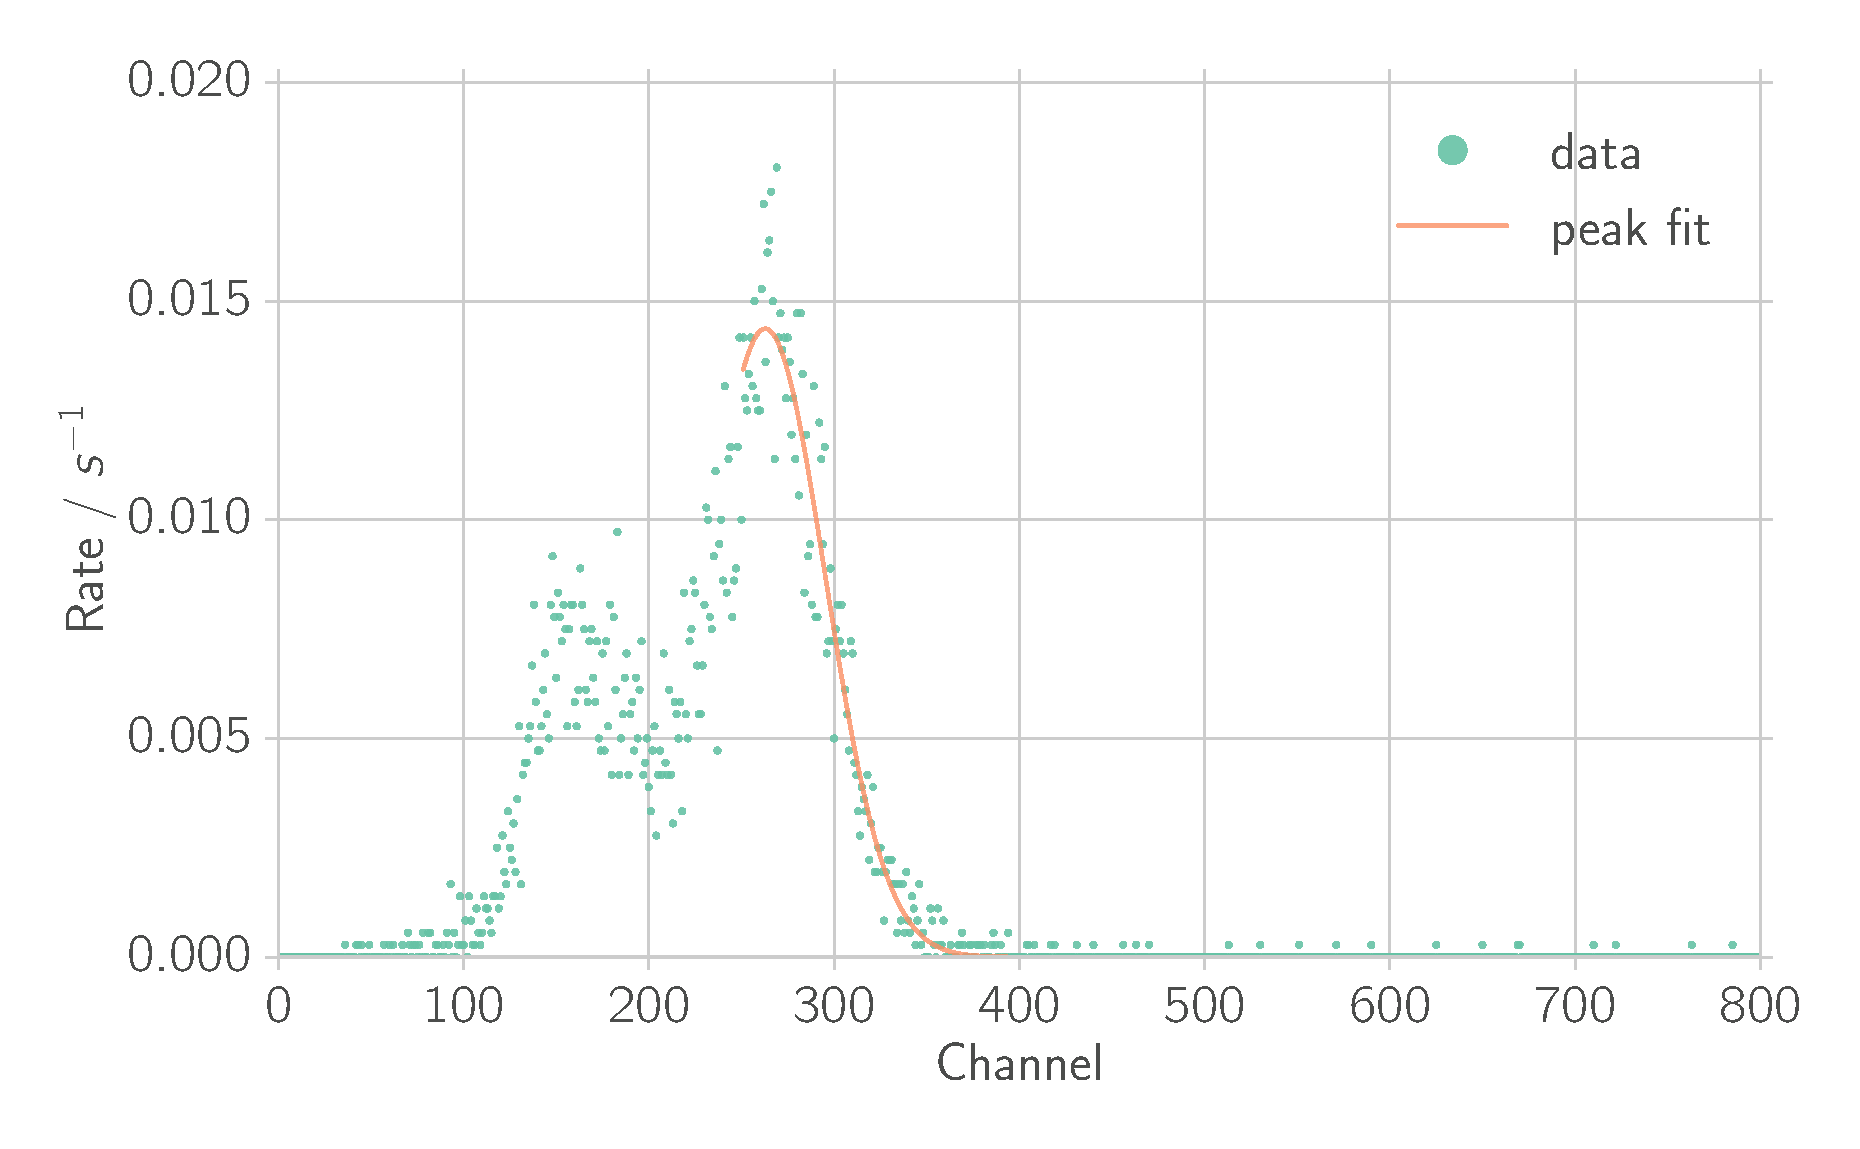
\includegraphics[width=0.9\linewidth]{./analysis/figures/coin_na_90}
\caption{\textbf{Energy of photons:} Rate of coincident events of 
        NaI scintillator at angle of $\theta = 90^\circ$. The distribution 
    was approximated with a Gaussian distribution. }
\label{fig:coin_na_90}
\end{figure}


\begin{figure}[htpb]
    \centering
    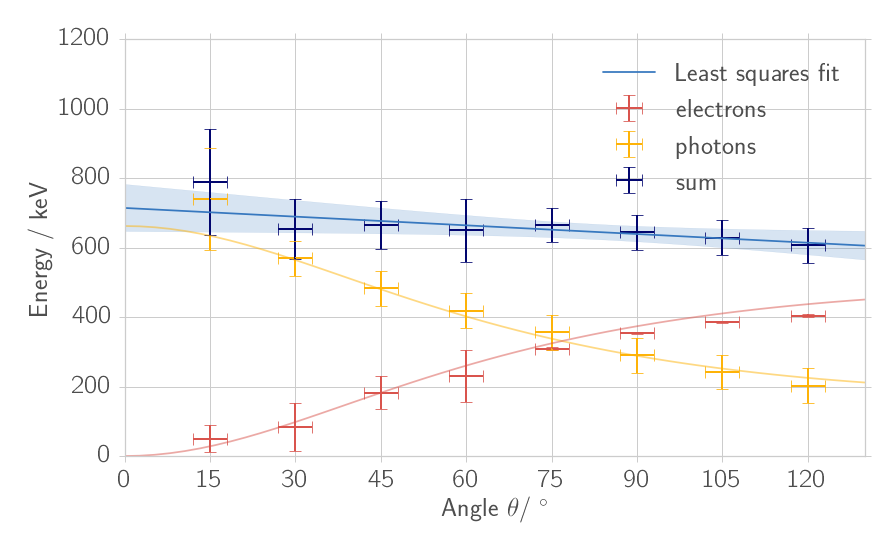
\includegraphics[width=0.9\linewidth]{./analysis/figures/energy_conservation}
    \caption{Summary of the analysis of the foregoing chapter. We note several aspects:
    The errors at small angles for the photon energies are rather high. 
    As result their weight in the fit will
    be rather small. Furthermore we arrive at a small tendency of a negative slope, which
    would disagree with energy conservation. However, this tendency is small, it is
    $[-0.7 \pm 0.8]$ keV/$^\circ$ where the height is $[750 \pm 80]$keV.}
\label{fig:energy_conservation}
\end{figure}



\clearpage
\section{Bibliography}
\printbibliography[heading=subbibintoc]
\clearpage

\end{document}
